\documentclass[aspectratio=169,11pt]{beamer}

% Shared style (ib-tutorials.sty at the repo root).
\makeatletter\def\input@path{{./}{../}}\makeatother
\usepackage{ib-tutorials}

\usepackage[utf8]{inputenc}
\usepackage{amsmath,amssymb}
\usepackage{booktabs}
\usepackage{array}
\newcolumntype{L}[1]{>{\raggedright\arraybackslash}p{#1}}
\usepackage{graphicx}
\usepackage{xcolor}
\usepackage{listings}
\usepackage{tikz}
\usetikzlibrary{arrows.meta,positioning,shapes.geometric,fit,calc}
\usepackage{hyperref}

\newcommand{\sourcecredit}[1]{\vfill\hfill{\tiny\textcolor{DarkGray}{#1}}}

\title[About these notes]{About these notes}
\subtitle{Where the material came from, who contributed, and what was left out}
\author[Miller]{Laura A. Miller}
\institute[UArizona]{Department of Mathematics, University of Arizona}
\date{Using IB Software \textbullet\ Part 0 \textbullet\ Chapter 0.1}

\begin{document}

% 1
\begin{frame}[plain]
\maketutorialtitlepanel{%
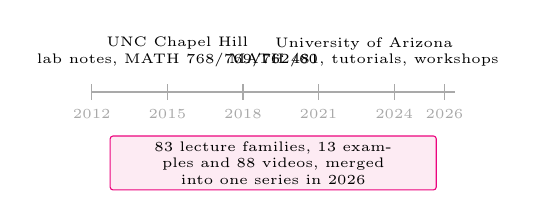
\begin{tikzpicture}[x=6.4mm]
  \draw[DarkGray,thick] (0,0) -- (7.2,0);
  \foreach \x/\y in {0/2012,1.5/2015,3/2018,4.5/2021,6/2024,7/2026}{
    \draw[DarkGray] (\x,-1mm) -- (\x,1mm);
    \node[font=\tiny,text=DarkGray,below=1mm] at (\x,0) {\y};}
  \node[font=\tiny,above=2mm,align=center] at (1.7,0) {UNC Chapel Hill\\lab notes, MATH 768/769/762/60};
  \node[font=\tiny,above=2mm,align=center] at (5.4,0) {University of Arizona\\MATH 481, tutorials, workshops};
  \node[draw=RubineRed,rounded corners=1pt,fill=RubineRed!8,font=\tiny,align=center,inner sep=2pt,text width=40mm] at (3.6,-9mm) {83 lecture families, 13 examples and 88 videos, merged into one series in 2026};
\end{tikzpicture}}
\end{frame}

% 2
\begin{frame}{What these notes are}
\begin{columns}[T,onlytextwidth]
\begin{column}{0.58\textwidth}
\textbf{Using IB Software} is one tutorial series on the practice of immersed boundary simulation:
\begin{itemize}
  \item \al{IB2d}: immersed boundary in 2D, in MATLAB or Python (Part II);
  \item \al{IBAMR}: immersed boundary in 2D and 3D on adaptive grids, in C++, including the finite element version \al{IBFE} (Parts III and IV);
  \item \al{VisIt}: looking at and analyzing the results (Part V);
  \item \al{Planktos}: agent-based models of organisms in the simulated flows (Part VI).
\end{itemize}
The companion series \textbf{Fluid Dynamics and IBM Theory} holds the equations, the discretization, and the solid mechanics behind the methods. These notes point to it and do not repeat it.
\end{column}
\begin{column}{0.40\textwidth}
\begin{punchbox}
\small Each chapter is one slide deck that starts with learning goals and ends with what can go wrong, a summary and references. Each worked example is a folder with tested code and a README that says what you should see.
\end{punchbox}
\vspace{2mm}
\small Written for students of the University of Arizona courses and for anyone starting with these codes. You should be comfortable with a terminal and have written some code in any language.
\end{column}
\end{columns}
\end{frame}

% 3
\begin{frame}{Where the material came from}
\scriptsize
\begin{tabular}{@{}L{0.12\textwidth}L{0.82\textwidth}@{}}
\toprule
2012--2013 & Miller lab IBAMR notes and ``Read Me'' decks at UNC Chapel Hill; MATH 769 (Spring 2013): IBAMR input files, boundary conditions, springs and targets, beams, forces, 3D, VisIt\\
2014 & \emph{IBAMR Tutorial: UNC Edition}; the first-simulation notes (ibamr-101); the IBFE tutorial series begins (meshes, PK1 stress, fiber tension); the gmsh geometry notes\\
2015 & MATH 769 (Spring 2015): changing parameters, VisIt in 3D; the VisIt data-analysis guide; meshing notes (CAD to STL to mesher)\\
2016--2017 & MATH 768 (2016) and MATH 60 (2017): IB2d and VisIt basics; gmsh 2D meshes from scratch; the IBFE series edited and extended (two meshes, 3D flow tank, advection--diffusion)\\
2018 & MATH 769 (Spring 2018): IBAMR part 1, IBFE, visualization and data analysis, shell scripting, all recorded; the two-coral target-point example in 3D\\
2019 & MATH 762: meshing, 3D scanning and finite elements; VisIt lectures re-recorded; the 2019 install notes\\
2020 & The Zoom lecture series (IBAMR 1--8, IBFE 1--8, VisIt 1--5): ConstraintIB, adding mass, Boyce's examples, main files; the move to the University of Arizona\\
2021--2022 & UA cluster notes (Ocelote, Puma); ib2d and IBAMR tutorials; the CFD course (MATH 481, Spring 2022: ANSYS, CAD, scanning); the IBFE summer meetings (autoibamr, Coreform Cubit)\\
2023--2024 & MATH 481 (ib2d, VisIt, validation); the 2023 VisIt tutorial videos; ``Write your own IBM code''; the 2024 summer tutorials; the AIMEC--NSF Cassiopea workshop (choosing software, building geometries); the Planktos decks\\
2025--2026 & IBAMR 0.16.0 installed on Puma with autoibamr; IBAMR 0.19.0 released; this consolidated series, with every example rebuilt and rerun\\
\bottomrule
\end{tabular}
\end{frame}

% 4
\begin{frame}{By the numbers}
\begin{columns}[T,onlytextwidth]
\begin{column}{0.5\textwidth}
\begin{itemize}
  \item About 150 slide decks, documents and example folders from the instructor's Google Drive, Dropbox and GitHub repositories, in several versions each.
  \item Grouped into \al{83 lecture families}; the newest or most complete version of each family became the basis of a chapter.
  \item \al{13 worked examples} (7 IB, 6 IBFE), each rebuilt with CMake and rerun with IBAMR 0.16.0 and 0.19.0; the course MATLAB scripts with Python versions.
  \item \al{88 lecture videos} (20.5 GB), listed on the following slides and not used.
\end{itemize}
\end{column}
\begin{column}{0.47\textwidth}
\begin{punchbox}
\small Nothing was thrown away. Material that no longer applies (retired clusters, old install recipes, old versions of the code) is in \textbf{Part X, Archive}, labelled \emph{legacy}, and the main chapters show the current way.
\end{punchbox}
\vspace{2mm}
\small The chapter decks are numbered 1--36 across Parts I--VII, with X1--X4 for the archive and A--C for the appendices. Chapter 0.2 is the map.
\end{column}
\end{columns}
\end{frame}

% 5
\begin{frame}{Contributors}
\footnotesize The notes were written and taught by Laura Miller. Many people contributed material, examples and tools over the years:
\scriptsize
\begin{columns}[T,onlytextwidth]
\begin{column}{0.5\textwidth}
\begin{itemize}\setlength{\itemsep}{0pt}
  \item \textbf{Boyce Griffith} (UNC): IBAMR itself, its examples and documentation, and the slides from which the overview of the IB method was adapted.
  \item \textbf{Alex Hoover}: the IBFE tutorial series (2014--2018): PK1 stress and body forces, fiber tension, creating meshes; the tube-heart and cluster examples.
  \item \textbf{Nick Battista}: IB2d and its documentation, the gmsh geometry tutorial (2014), and the notes on convergence.
  \item \textbf{Shannon Jones}: the 3D IBAMR notes (2012) and the video how-tos on visualizing finite element meshes and recording Python in VisIt.
  \item \textbf{Lindsay Waldrop}: the VisIt data-analysis guide (2015) and VisIt scripts.
  \item \textbf{Gabrielle Hobson}: post-processing IBAMR data in VisIt on a cluster (2020).
  \item \textbf{Dennis Evangelista}: the first-simulation notes (2014).
\end{itemize}
\end{column}
\begin{column}{0.48\textwidth}
\begin{itemize}\setlength{\itemsep}{0pt}
  \item \textbf{Austin Baird}: the lab's 2012--2013 IBAMR notes.
  \item \textbf{Julian Wag}: gmsh 2D meshes from scratch (2016) and example READMEs.
  \item \textbf{Matea Santiago}: the 2023 VisIt tutorial videos and MATH 481 material.
  \item \textbf{Christopher Strickland}: Planktos, and the Python readers for IBAMR output.
  \item \textbf{D. Michael Senter}: MeshmerizeMe, meshes from images for IB2d and IBAMR.
  \item \textbf{Eric Tytell}: the MATLAB toolbox for reading IBAMR output.
  \item The students and teaching assistants of every course, whose questions and mistakes shaped the ``what can go wrong'' slides.
\end{itemize}
Third-party material (vendor guides, other people's decks) is credited and linked where it is used, and was rewritten rather than copied.
\end{column}
\end{columns}
\end{frame}

% 6
\begin{frame}{How Claude was used}
\begin{columns}[T,onlytextwidth]
\begin{column}{0.5\textwidth}
\textbf{What Claude (Anthropic) did, in 2026}
\begin{itemize}
  \item read every version of every lecture, note and example;
  \item merged the versions of each topic into one chapter and rewrote the text in one voice and one format;
  \item checked the commands and the code against IBAMR 0.16.0 and 0.19.0, rebuilt the examples with CMake, ran them, and recorded what they do;
  \item drafted the slides and the example READMEs, and listed what was left out.
\end{itemize}
\end{column}
\begin{column}{0.48\textwidth}
\textbf{What is the instructor's}
\begin{itemize}
  \item the material itself: the course notes, the examples, the figures and movies, and the choices of what to teach and in what order;
  \item the review of each chapter before it enters the main branch of the repository.
\end{itemize}
\vspace{2mm}
\begin{punchbox}
\small The one-line disclosure at the bottom of every title slide says the same thing in short. If you find an error, open an issue on GitHub; the examples' READMEs say exactly what was run, so a wrong claim can be traced.
\end{punchbox}
\end{column}
\end{columns}
\end{frame}

% 7
\begin{frame}{What is not included}
\begin{itemize}
  \item \al{The lecture videos.} The 88 recordings from 2015 to 2024 (next three slides) are listed so that you know they exist. They are not part of these notes; new recordings will follow the new chapters.
  \item \al{Research codes} that are not teaching examples. Part VII says which research templates (insect wings, jellyfish, heart tubes, sea fans) are shared and which are not.
  \item \al{Other people's work}: student projects and theses, and third-party decks, which are cited rather than reproduced.
  \item \al{Private data} from the original notes: account names, passwords, e-mails and invoices were removed, and screenshots that showed them were replaced.
  \item \al{Non-IB software.} ANSYS, COMSOL and the CAD course are mentioned in chapter 1b for orientation and are not taught here.
  \item \al{Theory.} Derivations and the mathematics of the IB method moved to the companion series, \emph{Fluid Dynamics and IBM Theory}.
\end{itemize}
\end{frame}

% 8-10: the video list (generated by tools/video_frames.py)
% Generated by tools/video_frames.py from the video inventory. 88 videos.
\begin{frame}{Lecture videos (1 of 3)}
\tiny
The recordings below exist on the instructor's Drive (88 files, 20.5 GB in all) and are listed here only. They are not part of these notes, and new recordings will follow the new chapters. Sizes are in MB.
\vspace{1mm}
\begin{columns}[T,onlytextwidth]
\begin{column}{0.49\textwidth}
\begin{tabular}{@{}>{\raggedright\arraybackslash}p{0.66\linewidth}@{\hspace{3pt}}l@{\hspace{4pt}}r@{}}
\multicolumn{3}{@{}p{\linewidth}@{}}{\textbf{MATH 769 (Spring 2018): IBAMR part 1, getting started}}\\
2-\allowbreak{}UsingSakai-\allowbreak{}and-\allowbreak{}Killdevil.\allowbreak{}mp4 & 2018-01-24 & 332\\
3-\allowbreak{}Part1-\allowbreak{}IBAMR-\allowbreak{}Video-\allowbreak{}ElasticBoundary.\allowbreak{}mp4 & 2018-01-30 & 130\\
3-\allowbreak{}Part2-\allowbreak{}IBAMR-\allowbreak{}Video-\allowbreak{}ElasticBoundary.\allowbreak{}mp4 & 2018-01-30 & 164\\
4-\allowbreak{}InputBoundaryConditionsPart1.\allowbreak{}mp4 & 2018-02-05 & 160\\
4-\allowbreak{}InputBoundaryConditionsPart2.\allowbreak{}mp4 & 2018-02-05 & 202\\
4-\allowbreak{}InputBoundaryConditionsPart3.\allowbreak{}mp4 & 2018-02-05 & 197\\
5-\allowbreak{}Video-\allowbreak{}SpringsTargetsPart1.\allowbreak{}mp4 & 2018-02-14 & 250\\
5-\allowbreak{}Video-\allowbreak{}SpringsTargetsPart2.\allowbreak{}mp4 & 2018-02-14 & 240\\
2-\allowbreak{}FirstIBAMRSimlation.\allowbreak{}mov & 2018-02-23 & 682\\
6-\allowbreak{}Video\_\allowbreak{}IBAMRTutorial\_\allowbreak{}MultipleBoundaries\_\allowbreak{}DomainSize\_\allowbreak{}InputFile.\allowbreak{}mp4 & 2018-03-19 & 229\\
6-\allowbreak{}Video\_\allowbreak{}IBAMRTutorial\_\allowbreak{}MultipleBoundaries\_\allowbreak{}DomainSize\_\allowbreak{}InputFilePart2.\allowbreak{}mp4 & 2018-03-19 & 172\\
2-\allowbreak{}Video\_\allowbreak{}IBAMRTutorial\_\allowbreak{}RunOnDogwood.\allowbreak{}mp4 & 2018-04-13 & 638\\
\multicolumn{3}{@{}p{\linewidth}@{}}{\textbf{MATH 769 (2018): IBFE}}\\
1-\allowbreak{}Video\_\allowbreak{}IBFE\_\allowbreak{}GettingStarted.\allowbreak{}mp4 & 2018-04-13 & 451\\
3-\allowbreak{}Video\_\allowbreak{}IBFE\_\allowbreak{}MakeMeshandMoveIt.\allowbreak{}mp4 & 2018-04-13 & 728\\
3B-\allowbreak{}Video\_\allowbreak{}IBFE\_\allowbreak{}RecordPythonandRunPart1.\allowbreak{}mp4 & 2018-04-16 & 614\\
3B-\allowbreak{}Video\_\allowbreak{}IBFE\_\allowbreak{}RecordPythonandRun\_\allowbreak{}Part2.\allowbreak{}mp4 & 2018-04-16 & 549\\
\end{tabular}
\end{column}
\begin{column}{0.49\textwidth}
\begin{tabular}{@{}>{\raggedright\arraybackslash}p{0.66\linewidth}@{\hspace{3pt}}l@{\hspace{4pt}}r@{}}
\multicolumn{3}{@{}p{\linewidth}@{}}{\textbf{MATH 769 (2018): lectures on FSI in biology}}\\
1-\allowbreak{}Introduction2IBM-\allowbreak{}NumericalConsiderations.\allowbreak{}mp4 & 2018-01-24 & 841\\
2-\allowbreak{}IntroDimensionlessParameters.\allowbreak{}mp4 & 2018-02-11 & 501\\
\multicolumn{3}{@{}p{\linewidth}@{}}{\textbf{MATH 769 (2018): professional development}}\\
LiteratureSearchPart1.\allowbreak{}mp4 & 2018-02-11 & 346\\
LiteratureSearchPart2.\allowbreak{}mp4 & 2018-02-11 & 235\\
\multicolumn{3}{@{}p{\linewidth}@{}}{\textbf{Visualization and data analysis (2018--2019)}}\\
2-\allowbreak{}Video\_\allowbreak{}Visualizing3Ddata.\allowbreak{}mp4 & 2018-02-26 & 258\\
4-\allowbreak{}Video\_\allowbreak{}VisitDataAnalysis-\allowbreak{}SamplingandTimeQueries.\allowbreak{}mp4 & 2018-03-19 & 323\\
4-\allowbreak{}Video\_\allowbreak{}VisitDataAnalysis-\allowbreak{}SamplingandTimeQueriesPart2.\allowbreak{}mp4 & 2018-03-19 & 208\\
5-\allowbreak{}Video\_\allowbreak{}IBAMR\_\allowbreak{}MATLAB\_\allowbreak{}Analysis\_\allowbreak{}Part1.\allowbreak{}mp4 & 2018-03-19 & 219\\
5-\allowbreak{}Video\_\allowbreak{}IBAMR\_\allowbreak{}MATLAB\_\allowbreak{}Analysis\_\allowbreak{}Part2.\allowbreak{}mp4 & 2018-03-19 & 370\\
6-\allowbreak{}Video\_\allowbreak{}ResamplingAMR2UniformGrid\_\allowbreak{}Exporting2vtk\_\allowbreak{}RecordingInPython.\allowbreak{}mp4 & 2018-03-19 & 523\\
7-\allowbreak{}Video\_\allowbreak{}IBAMR\_\allowbreak{}RunningManySims1A\_\allowbreak{}Intro2ShellScripting.\allowbreak{}mp4 & 2018-03-25 & 523\\
7-\allowbreak{}Video\_\allowbreak{}IBAMR\_\allowbreak{}RunningManySims1B\_\allowbreak{}Intro2ShellScripting.\allowbreak{}mp4 & 2018-03-25 & 662\\
7-\allowbreak{}Video\_\allowbreak{}IBAMR\_\allowbreak{}RunningManySimsPart2\_\allowbreak{}Intro2ShellScripting.\allowbreak{}mp4 & 2018-04-02 & 738\\
8-\allowbreak{}Visit from command line and Python.\allowbreak{}mp4 & 2018-04-02 & 809\\
\end{tabular}
\end{column}
\end{columns}
\end{frame}

\begin{frame}{Lecture videos (2 of 3)}
\tiny
\begin{columns}[T,onlytextwidth]
\begin{column}{0.49\textwidth}
\begin{tabular}{@{}>{\raggedright\arraybackslash}p{0.66\linewidth}@{\hspace{3pt}}l@{\hspace{4pt}}r@{}}
1-\allowbreak{}2DVisitVisualization.\allowbreak{}mp4 & 2019-10-23 & 471\\
\multicolumn{3}{@{}p{\linewidth}@{}}{\textbf{2019 VisIt lectures}}\\
Lecture 1-\allowbreak{}2DVisitVisualization.\allowbreak{}mp4 & 2019-07-03 & 471\\
Lecture 2-\allowbreak{}Video\_\allowbreak{}Visualizing3Ddata.\allowbreak{}mp4 & 2019-07-03 & 258\\
\multicolumn{3}{@{}p{\linewidth}@{}}{\textbf{2020 Zoom lectures (IBAMR, IBFE, VisIt)}}\\
Lecture 1 -\allowbreak{} Running your first simulation.\allowbreak{}mp4 & 2020-05-11 & 93\\
Visualization Lecture 1 -\allowbreak{} Getting Started with VisIt.\allowbreak{}mp4 & 2020-05-12 & 125\\
Lecture 2 -\allowbreak{} Intro to IBM.\allowbreak{}mp4 & 2020-05-13 & 91\\
Lecture 3 -\allowbreak{} IBAMR input files.\allowbreak{}mp4 & 2020-05-14 & 104\\
Lecture 4 -\allowbreak{} Boundary conditions, domain sizes, etc.\allowbreak{}.\allowbreak{}mp4 & 2020-05-15 & 70\\
Lecture 5 -\allowbreak{} Moving immersed boundaries.\allowbreak{}mp4 & 2020-05-19 & 69\\
IBFE-\allowbreak{}Lecture1-\allowbreak{}BeamExample.\allowbreak{}mp4 & 2020-05-20 & 63\\
IBFE-\allowbreak{}Lecture2-\allowbreak{}MakeYourOwnMesh.\allowbreak{}mp4 & 2020-05-26 & 77\\
IBFE-\allowbreak{}Lectures 3 and 4 -\allowbreak{} Active stresses.\allowbreak{}mp4 & 2020-05-27 & 77\\
IBFE-\allowbreak{}Lecture5 -\allowbreak{} Plans for June.\allowbreak{}mov & 2020-06-01 & 69\\
Lecture 6 -\allowbreak{} What do Boyce\textquotesingle{}s examples do.\allowbreak{}mp4 & 2020-07-21 & 58\\
IBFE-\allowbreak{}Lecture7-\allowbreak{}TwoBoundaries.\allowbreak{}mp4 & 2020-08-10 & 40\\
IBFE-\allowbreak{}Lecture 8 -\allowbreak{} Main Files.\allowbreak{}mp4 & 2020-09-01 & 73\\
\end{tabular}
\end{column}
\begin{column}{0.49\textwidth}
\begin{tabular}{@{}>{\raggedright\arraybackslash}p{0.66\linewidth}@{\hspace{3pt}}l@{\hspace{4pt}}r@{}}
Lecture 7 -\allowbreak{} Constraint IB with Sound.\allowbreak{}mp4 & 2020-09-09 & 50\\
Lecture 7 -\allowbreak{} No Sound -\allowbreak{} Constraint IB.\allowbreak{}mp4 & 2020-09-09 & 118\\
Visualization Lecture 5 -\allowbreak{} Visit on the cluster.\allowbreak{}mp4 & 2020-09-23 & 81\\
Lecture 8 -\allowbreak{} Adding massive points.\allowbreak{}mp4 & 2020-11-11 & 42\\
IBFE-\allowbreak{}Lectures 3 and 4 -\allowbreak{} Active stresses.\allowbreak{}mp4 & 2021-06-25 & 77\\
Hamlet\_\allowbreak{}Run\_\allowbreak{}IBAMR.\allowbreak{}mp4 & 2021-08-04 & 9\\
\multicolumn{3}{@{}p{\linewidth}@{}}{\textbf{2020, other}}\\
Gmsh2D.\allowbreak{}mp4 & 2020-10-02 & 37\\
\multicolumn{3}{@{}p{\linewidth}@{}}{\textbf{2022 CFD course (ANSYS, CAD, Meshmixer; not IB software)}}\\
Tutorial1-\allowbreak{}ANSYSandIBAMR.\allowbreak{}mp4 & 2022-01-18 & 367\\
Tutorial3 -\allowbreak{} Meshmixer.\allowbreak{}mp4 & 2022-02-04 & 372\\
Tutorial4A -\allowbreak{} Cleaning Meshes.\allowbreak{}mp4 & 2022-02-15 & 372\\
Tutorial4B-\allowbreak{}MeshCleaningANSYSsimulation.\allowbreak{}mp4 & 2022-02-15 & 309\\
Tutorial2 -\allowbreak{} Autodesk Fusion.\allowbreak{}mp4 & 2022-02-24 & 343\\
ANSYSQuickOverviewTrachea.\allowbreak{}mp4 & 2022-04-21 & 176\\
\multicolumn{3}{@{}p{\linewidth}@{}}{\textbf{2022 IBFE summer meetings}}\\
July-\allowbreak{}21-\allowbreak{}2022-\allowbreak{}Installing-\allowbreak{}autoibamr.\allowbreak{}mp4 & 2022-07-21 & 157\\
\end{tabular}
\end{column}
\end{columns}
\end{frame}

\begin{frame}{Lecture videos (3 of 3)}
\tiny
\begin{columns}[T,onlytextwidth]
\begin{column}{0.49\textwidth}
\begin{tabular}{@{}>{\raggedright\arraybackslash}p{0.66\linewidth}@{\hspace{3pt}}l@{\hspace{4pt}}r@{}}
June-\allowbreak{}23-\allowbreak{}2022-\allowbreak{}InitialMeetingOverview.\allowbreak{}mp4 & 2022-07-21 & 306\\
June-\allowbreak{}30-\allowbreak{}2022-\allowbreak{}QuickActiveTensionReview.\allowbreak{}mp4 & 2022-07-21 & 97\\
July-\allowbreak{}28-\allowbreak{}2022-\allowbreak{}Coreform-\allowbreak{}Tutorial.\allowbreak{}mp4 & 2022-07-29 & 345\\
\multicolumn{3}{@{}p{\linewidth}@{}}{\textbf{2022 ib2d and IBAMR tutorials}}\\
Tutorial2-\allowbreak{}Boundaries-\allowbreak{}ib2d-\allowbreak{}IBAMR.\allowbreak{}mp4 & 2022-01-28 & 240\\
Tutorial3-\allowbreak{}MovingBoundaries-\allowbreak{}ib2d.\allowbreak{}mp4 & 2022-02-04 & 128\\
Tutorial1B-\allowbreak{}RunningIBAMR.\allowbreak{}mp4 & 2022-02-24 & 161\\
GenerateMeshTutorialPart1.\allowbreak{}mp4 & 2022-04-21 & 182\\
GenerateMeshTutorialPart2.\allowbreak{}mp4 & 2022-04-21 & 267\\
\multicolumn{3}{@{}p{\linewidth}@{}}{\textbf{2023 VisIt tutorial (M. Santiago)}}\\
2D Slices.\allowbreak{}mp4 & 2023-07-25 & 61\\
3D flow.\allowbreak{}mp4 & 2023-07-25 & 40\\
Finalizing Visualizations.\allowbreak{}mp4 & 2023-07-25 & 48\\
Intro-\allowbreak{}Mesh-\allowbreak{}Body.\allowbreak{}mp4 & 2023-07-25 & 18\\
\multicolumn{3}{@{}p{\linewidth}@{}}{\textbf{2023 ``Write your own IBM code'' (a simulation movie)}}\\
fluid\_\allowbreak{}movie\_\allowbreak{}16.\allowbreak{}avi & 2023-05-07 & 9\\
\multicolumn{3}{@{}p{\linewidth}@{}}{\textbf{2024 summer tutorials: IBAMR}}\\
IBAMR-\allowbreak{}BCs-\allowbreak{}July11.\allowbreak{}mp4 & 2024-07-11 & 131\\
\end{tabular}
\end{column}
\begin{column}{0.49\textwidth}
\begin{tabular}{@{}>{\raggedright\arraybackslash}p{0.66\linewidth}@{\hspace{3pt}}l@{\hspace{4pt}}r@{}}
IBAMR-\allowbreak{}DomainSize-\allowbreak{}July16.\allowbreak{}mp4 & 2024-07-16 & 233\\
IBAMR-\allowbreak{}intro-\allowbreak{}running-\allowbreak{}on-\allowbreak{}hpc-\allowbreak{}July3.\allowbreak{}mp4 & 2024-07-16 & 243\\
IBAMR-\allowbreak{}MovingTarget-\allowbreak{}ChangeSprings.\allowbreak{}mp4 & 2024-07-28 & 201\\
\multicolumn{3}{@{}p{\linewidth}@{}}{\textbf{2024 summer tutorials: IBFE}}\\
0-\allowbreak{}IBFE-\allowbreak{}Getting-\allowbreak{}Started.\allowbreak{}mp4 & 2024-08-01 & 121\\
1-\allowbreak{}IBFE-\allowbreak{}TargetPlateExample.\allowbreak{}mp4 & 2024-08-01 & 355\\
2-\allowbreak{}IBFE-\allowbreak{}MakeMeshMoveIt.\allowbreak{}mp4 & 2024-08-01 & 67\\
\multicolumn{3}{@{}p{\linewidth}@{}}{\textbf{2024 summer tutorials: ib2d}}\\
ib2d-\allowbreak{}intro-\allowbreak{}07-\allowbreak{}02-\allowbreak{}2024.\allowbreak{}mp4 & 2024-07-02 & 250\\
\multicolumn{3}{@{}p{\linewidth}@{}}{\textbf{2015 tube-heart simulation movies (lab project; not lectures)}}\\
tubemovie\_\allowbreak{}oneactivation.\allowbreak{}mpg & 2015-08-21 & 4\\
tubemovie\_\allowbreak{}1hz\_\allowbreak{}activation.\allowbreak{}mpg & 2015-08-24 & 7\\
tubemovie\_\allowbreak{}1hz\_\allowbreak{}activation\_\allowbreak{}altview.\allowbreak{}mpg & 2015-08-24 & 3\\
tubemovie\_\allowbreak{}oneactivation\_\allowbreak{}altview\_\allowbreak{}mu1e5\_\allowbreak{}T2e5.\allowbreak{}mpg & 2015-08-27 & 3\\
tubemovie\_\allowbreak{}oneactivation\_\allowbreak{}mu1e5\_\allowbreak{}T2e5.\allowbreak{}mpg & 2015-08-27 & 7\\
tubemovie\_\allowbreak{}peristalsis\_\allowbreak{}altview\_\allowbreak{}mu1e6\_\allowbreak{}T1e6.\allowbreak{}mpg & 2015-10-19 & 3\\
tubemovie\_\allowbreak{}peristalsis\_\allowbreak{}mu1e6\_\allowbreak{}T1e6.\allowbreak{}mpg & 2015-10-19 & 6\\
\end{tabular}
\end{column}
\end{columns}
\end{frame}


% 11
\begin{frame}{License, citation and where things are}
\footnotesize
\begin{columns}[T,onlytextwidth]
\begin{column}{0.5\textwidth}
\textbf{License}
\begin{itemize}
  \item Text, slides and figures: Creative Commons Attribution 4.0 (CC BY 4.0).
  \item Code in \code{examples/}: BSD 3-Clause.
  \item Third-party items keep their own licenses, named where they appear.
\end{itemize}
\vspace{1mm}
\textbf{To cite these notes}\\
Miller, L. A. (2026). \emph{Using IB Software: tutorials for IB2d, IBAMR, VisIt and Planktos.} \url{https://github.com/fairyflies9/Using-IB-Software}
\end{column}
\begin{column}{0.48\textwidth}
\textbf{Where things are}
\begin{itemize}
  \item These notes: \url{https://github.com/fairyflies9/Using-IB-Software}
  \item The theory series: \url{https://github.com/equiphysics/Fluid-Dynamics-and-IBM-Theory}
  \item IBAMR: \url{https://ibamr.github.io}
  \item IB2d: \url{https://github.com/nickabattista/IB2d}
  \item VisIt: \url{https://visit-dav.github.io/visit-website/}
  \item Planktos: \url{https://github.com/mountaindust/Planktos}
\end{itemize}
\begin{homebox}
Next, chapter 0.2: the map of the chapters, the software versions used, and where the examples live.
\end{homebox}
\end{column}
\end{columns}
\end{frame}

\end{document}
